\documentclass{beamer}
\mode<presentation>
\usepackage{amsmath,amssymb,mathtools}
\usepackage{textcomp}
\usepackage{gensymb}
\usepackage{adjustbox}
\usepackage{subcaption}
\usepackage{enumitem}
\usepackage{multicol}
\usepackage{listings}
\usepackage{url}
\usepackage{graphicx} % <-- needed for images
\def\UrlBreaks{\do\/\do-}

\usetheme{Boadilla}
\usecolortheme{lily}
\setbeamertemplate{footline}{
  \leavevmode%
  \hbox{%
  \begin{beamercolorbox}[wd=\paperwidth,ht=2ex,dp=1ex,right]{author in head/foot}%
    \insertframenumber{} / \inserttotalframenumber\hspace*{2ex}
  \end{beamercolorbox}}%
  \vskip0pt%
}
\setbeamertemplate{navigation symbols}{}

\lstset{
  frame=single,
  breaklines=true,
  columns=fullflexible,
  basicstyle=\ttfamily\tiny   % tiny font so code fits
}

\numberwithin{equation}{section}

% ---- your macros ----
\providecommand{\nCr}[2]{\,^{#1}C_{#2}}
\providecommand{\nPr}[2]{\,^{#1}P_{#2}}
\providecommand{\mbf}{\mathbf}
\providecommand{\pr}[1]{\ensuremath{\Pr\left(#1\right)}}
\providecommand{\qfunc}[1]{\ensuremath{Q\left(#1\right)}}
\providecommand{\sbrak}[1]{\ensuremath{{}\left[#1\right]}}
\providecommand{\lsbrak}[1]{\ensuremath{{}\left[#1\right.}}
\providecommand{\rsbrak}[1]{\ensuremath{\left.#1\right]}}
\providecommand{\brak}[1]{\ensuremath{\left(#1\right)}}
\providecommand{\lbrak}[1]{\ensuremath{\left(#1\right.}}
\providecommand{\rbrak}[1]{\ensuremath{\left.#1\right)}}
\providecommand{\cbrak}[1]{\ensuremath{\left\{#1\right\}}}
\providecommand{\lcbrak}[1]{\ensuremath{\left\{#1\right.}}
\providecommand{\rcbrak}[1]{\ensuremath{\left.#1\right\}}}
\theoremstyle{remark}
\newtheorem{rem}{Remark}
\newcommand{\sgn}{\mathop{\mathrm{sgn}}}
\providecommand{\abs}[1]{\left\vert#1\right\vert}
\providecommand{\res}[1]{\Res\displaylimits_{#1}}
\providecommand{\norm}[1]{\lVert#1\rVert}
\providecommand{\mtx}[1]{\mathbf{#1}}
\providecommand{\mean}[1]{E\left[ #1 \right]}
\providecommand{\fourier}{\overset{\mathcal{F}}{ \rightleftharpoons}}
\providecommand{\system}{\overset{\mathcal{H}}{ \longleftrightarrow}}
\providecommand{\dec}[2]{\ensuremath{\overset{#1}{\underset{#2}{\gtrless}}}}
\newcommand{\myvec}[1]{\ensuremath{\begin{pmatrix}#1\end{pmatrix}}}
\let\vec\mathbf
% ---------------------

\title{Matgeo Presentation - Problem 2.4.16}
\author{ee25btech11021 - Dhanush sagar}

\begin{document}
	

		




%---------------- Title Page ----------------
\begin{frame}
  \titlepage
\end{frame}

%---------------- Problem Statement ----------------
\begin{frame}{Problem Statement}
 Verify the following:\\  
(a) $(0,7,-10), (1,6,-6)$ and $(4,9,-6)$ are the vertices of an isosceles triangle.  \\
(b) $(0,7,10), (-1,6,6)$ and $(-4,9,6)$ are the vertices of a right-angled triangle.
\end{frame}

%---------------- Mathematical Formula ----------------
\begin{frame}{solution}
 

\textbf{Solution a}\\
% ---------- Part (a) ----------
\textbf{Property:} In an isosceles triangle, the perpendicular bisector of a side passes through the opposite vertex.

\begin{align}
\vec{A} = \myvec{0\\7\\-10},  
\vec{B} = \myvec{1\\6\\-6},  
\vec{C} = \myvec{4\\9\\-6}
\end{align}
\text{Midpoint of side } AC: 
\begin{align}
 \vec{M} = \frac{\vec{A}+\vec{C}}{2} 
= \frac{\myvec{0\\7\\-10}+\myvec{4\\9\\-6}}{2} 
= \myvec{2\\8\\-8}
\end{align}
\text{Direction vector of side } AC: 
\begin{align}
 \vec{C}-\vec{A} = \myvec{4\\9\\-6}-\myvec{0\\7\\-10} 
= \myvec{4\\2\\4}
\end{align}
\end{frame}
\begin{frame}{solution}
\text{Vector from midpoint to } B:
\begin{align}
\vec{B}-\vec{M} = \myvec{1\\6\\-6}-\myvec{2\\8\\-8} 
= \myvec{-1\\-2\\2}
\end{align}
\begin{align}
(\vec{C}-\vec{A})^\top(\vec{B}-\vec{M}) 
= \myvec{4&2&4}\myvec{-1\\-2\\2} = -4-4+8=0
\end{align}
\begin{align*}
 \vec{B} \text{ lies on the perpendicular bisector of side } AC.\\
 \therefore AB = BC \implies \triangle ABC \text{ is isosceles.}
\end{align*}
\textbf{Solution b}\\
\textbf{Property:} If two sides of a triangle are perpendicular, then the included angle is a right angle.
\begin{align}
\vec{A} = \myvec{0\\7\\10},  
\vec{B} = \myvec{-1\\6\\6},  
\vec{C} = \myvec{-4\\9\\6}
\end{align}
\end{frame}
\begin{frame}{solution}
\begin{align}
\vec{A}-\vec{B} = \myvec{0\\7\\10}-\myvec{-1\\6\\6} 
= \myvec{1\\1\\4}
\end{align}
\begin{align}
\vec{C}-\vec{B} = \myvec{-4\\9\\6}-\myvec{-1\\6\\6} 
= \myvec{-3\\3\\0}
\end{align}
\begin{align}
(\vec{A}-\vec{B})^\top(\vec{C}-\vec{B}) 
= \myvec{1&1&4}\myvec{-3\\3\\0} = -3+3+0=0
\end{align}
\begin{align*}
\implies \vec{A}-\vec{B} \perp \vec{C}-\vec{B}  \Rightarrow  
\triangle ABC \text{ is right-angled at } B.
\end{align*}



\end{frame}
%---------------- C Source Code ----------------
\begin{frame}[fragile]{C Source Code:gen point.c}
\begin{verbatim}

#include <stdio.h>

// Function to write first set of points (isosceles triangle)
void generate_points_isosceles(const char *filename) {
    FILE *fp = fopen(filename, "w");
    if (fp == NULL) {
        printf("Error opening file!\n");
        return;
    }

    double A[3] = {0, 7, -10};
    double B[3] = {1, 6, -6};
    double C[3] = {4, 9, -6};
   
\end{verbatim}
\end{frame}
\begin{frame}[fragile]{C Source Code:gen point.c}
\begin{verbatim}
    fprintf(fp, "%lf %lf %lf\n", A[0], A[1], A[2]);
    fprintf(fp, "%lf %lf %lf\n", B[0], B[1], B[2]);
    fprintf(fp, "%lf %lf %lf\n", C[0], C[1], C[2]);
    fclose(fp);
}

// Function to write second set of points (right-angled triangle)
void generate_points_right(const char *filename) {
    FILE *fp = fopen(filename, "w");
    if (fp == NULL) {
        printf("Error opening file!\n");
        return;
    }

\end{verbatim}
\end{frame}

%---------------- Python solve.py ----------------
\begin{frame}[fragile]{Python Script: solve triangle.py}
\begin{verbatim}


import ctypes
import numpy as np

# Load shared object
lib = ctypes.CDLL("./gen_points.so")

# Call C functions
lib.generate_points_isosceles(b"iso_points.dat")
lib.generate_points_right(b"right_points.dat")

# Load points
iso_points = np.loadtxt("iso_points.dat")
right_points = np.loadtxt("right_points.dat")
\end{verbatim}
\end{frame}
\begin{frame}[fragile]{Python Script: solve triangle.py}
\begin{verbatim}
# Distance squared function
def dist2(P, Q):
    return np.sum((P - Q) ** 2)

# --------- Part (a) Isosceles Triangle -----------
A, B, C = iso_points
AB2 = dist2(A, B)
BC2 = dist2(B, C)
CA2 = dist2(C, A)

print("Isosceles Triangle Check:")
print("AB^2 =", AB2, "BC^2 =", BC2, "CA^2 =", CA2)
isosceles = (AB2 == BC2) or (BC2 == CA2) or (CA2 == AB2)
print("Isosceles:", isosceles)
print()
\end{verbatim}
\end{frame}
\begin{frame}[fragile]{Python Script: solve triangle.py}
\begin{verbatim}
# --------- Part (b) Right Angled Triangle ---------
P, Q, R = right_points
PQ2 = dist2(P, Q)
QR2 = dist2(Q, R)
RP2 = dist2(R, P)

print("Right Angled Triangle Check:")
print("PQ^2 =", PQ2, "QR^2 =", QR2, "RP^2 =", RP2)
right_angle = (PQ2 + QR2 == RP2) or (QR2 + RP2 == PQ2) or (RP2 + PQ2 == QR2)
print("Right Angled:", right_angle)

\end{verbatim}
\end{frame}

%---------------- Python plot.py ----------------
\begin{frame}[fragile]{Python Script: plot triangle.py}
\begin{verbatim}
import sys
sys.path.insert(0,  '/home/dhanush-sagar/matgeo/codes/CoordGeo')
import numpy as np
import matplotlib.pyplot as plt


# Local imports
from line.funcs import *
from triangle.funcs import *
from conics.funcs import circ_gen

# Load both sets of points
iso_points = np.loadtxt("iso_points.dat")
right_points = np.loadtxt("right_points.dat")

# ---- Plot Isosceles Triangle ----
fig1 = plt.figure()
\end{verbatim}
\end{frame}
\begin{frame}[fragile]{Python Script: plot triangle.py}
\begin{verbatim}
ax1 = fig1.add_subplot(111, projection='3d')
A, B, C = iso_points
tri_iso = np.vstack((A, B, C, A))
ax1.plot(tri_iso[:,0], tri_iso[:,1], tri_iso[:,2], 'b-o', label='Isosceles Triangle')
ax1.text(A[0], A[1], A[2], "A", color='red')
ax1.text(B[0], B[1], B[2], "B", color='red')
ax1.text(C[0], C[1], C[2], "C", color='red')
ax1.set_title("Isosceles Triangle")
ax1.set_xlabel("X-axis")
ax1.set_ylabel("Y-axis")
ax1.set_zlabel("Z-axis")
plt.legend()
plt.savefig("isosceles_triangle.png")
plt.show()

# ---- Plot Right-Angled Triangle ----
fig2 = plt.figure()
\end{verbatim}
\end{frame}
\begin{frame}[fragile]{Python Script: plot triangle.py}
\begin{verbatim}
ax2 = fig2.add_subplot(111, projection='3d')
P, Q, R = right_points
tri_right = np.vstack((P, Q, R, P))
ax2.plot(tri_right[:,0], tri_right[:,1], tri_right[:,2], 'g-o', label='Right-Angled Triangle')
ax2.text(P[0], P[1], P[2], "P", color='red')
ax2.text(Q[0], Q[1], Q[2], "Q", color='red')
ax2.text(R[0], R[1], R[2], "R", color='red')
ax2.set_title("Right-Angled Triangle")
ax2.set_xlabel("X-axis")
ax2.set_ylabel("Y-axis")
ax2.set_zlabel("Z-axis")
plt.legend()
plt.savefig("right_triangle.png")
plt.show()


\end{verbatim}
\end{frame}

%---------------- Result Plot ----------------
\begin{frame}{Result Plot}
 \begin{figure}[H]
     \centering
     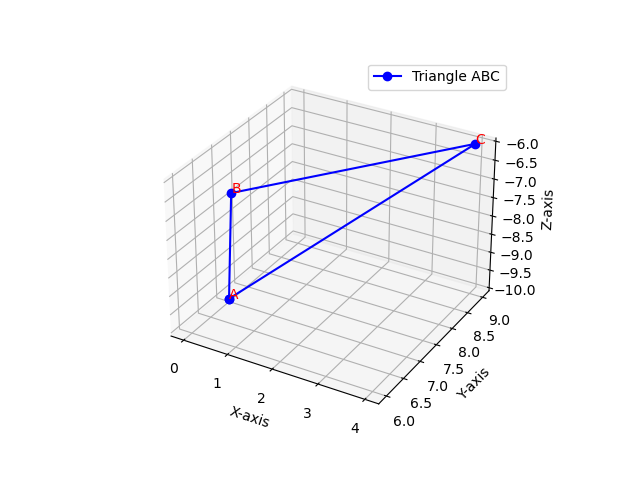
\includegraphics[width=0.8\columnwidth]{figs/fig1.png}
     \caption*{}
     \label{fig:fig1}
 \end{figure}
  
\end{frame}
\begin{frame}{Result Plot}
 \begin{figure}[H]
     \centering
     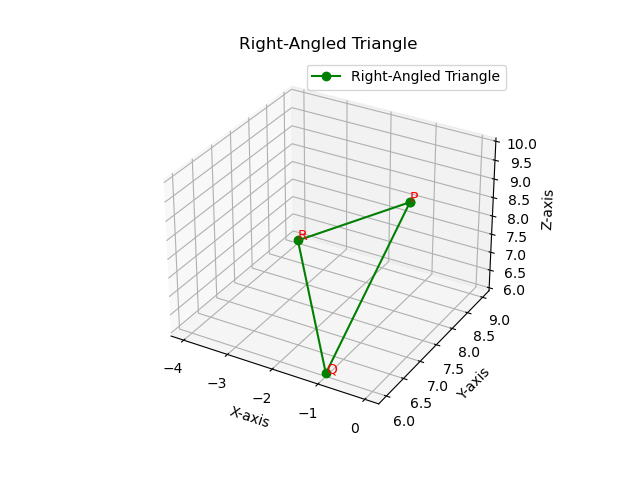
\includegraphics[width=0.8\columnwidth]{figs/fig2.png}
     \caption*{}
     \label{fig:fig1}
 \end{figure}
  
\end{frame}
\end{document}
